\hypertarget{_trace_line_8c}{
\section{/home/mgh/LanlGeoMag/libLanlGeoMag/TraceLine.c File Reference}
\label{_trace_line_8c}\index{/home/mgh/LanlGeoMag/libLanlGeoMag/TraceLine.c@{/home/mgh/LanlGeoMag/libLanlGeoMag/TraceLine.c}}
}
{\tt \#include $<$stdio.h$>$}\par
{\tt \#include $<$stdlib.h$>$}\par
{\tt \#include \char`\"{}Lgm/Lgm\_\-MagModelInfo.h\char`\"{}}\par


Include dependency graph for TraceLine.c:\nopagebreak
\begin{figure}[H]
\begin{center}
\leavevmode
\includegraphics[width=387pt]{_trace_line_8c__incl}
\end{center}
\end{figure}
\subsection*{Defines}
\begin{CompactItemize}
\item 
\#define \hyperlink{_trace_line_8c_d0c1d45514a182c1e2165de7582e96db}{GSL\_\-INTERP}~gsl\_\-interp\_\-cspline
\end{CompactItemize}
\subsection*{Functions}
\begin{CompactItemize}
\item 
int \hyperlink{_trace_line_8c_3683689fb880f54289fd4600f8b7dfc9}{Lgm\_\-TraceLine} (\hyperlink{struct_lgm___vector}{Lgm\_\-Vector} $\ast$u, \hyperlink{struct_lgm___vector}{Lgm\_\-Vector} $\ast$v, double H0, double sgn, double tol, int AddBminPoint, \hyperlink{struct_lgm___mag_model_info}{Lgm\_\-MagModelInfo} $\ast$Info)
\item 
int \hyperlink{_trace_line_8c_603527e81ecde7cb9495efc9bcb6d386}{Lgm\_\-TraceLine2} (\hyperlink{struct_lgm___vector}{Lgm\_\-Vector} $\ast$u, \hyperlink{struct_lgm___vector}{Lgm\_\-Vector} $\ast$v, double H0, double MinDist, double sgn, double tol, int AddBminPoint, \hyperlink{struct_lgm___mag_model_info}{Lgm\_\-MagModelInfo} $\ast$Info)
\item 
void \hyperlink{_trace_line_8c_069290bbefbad1db8e625b9e8a0d3a5e}{ReplaceFirstPoint} (double s, double B, \hyperlink{struct_lgm___vector}{Lgm\_\-Vector} $\ast$P, \hyperlink{struct_lgm___mag_model_info}{Lgm\_\-MagModelInfo} $\ast$Info)
\item 
void \hyperlink{_trace_line_8c_a82612dffc3edae2b3fce7cb94e435c0}{AddNewPoint} (double s, double B, \hyperlink{struct_lgm___vector}{Lgm\_\-Vector} $\ast$P, \hyperlink{struct_lgm___mag_model_info}{Lgm\_\-MagModelInfo} $\ast$Info)
\item 
void \hyperlink{_trace_line_8c_a7175b98aed0d6f712ca66d532afe450}{InitSpline} (\hyperlink{struct_lgm___mag_model_info}{Lgm\_\-MagModelInfo} $\ast$Info)
\item 
void \hyperlink{_trace_line_8c_e748e444fc7e684dcead584e1d002e8d}{FreeSpline} (\hyperlink{struct_lgm___mag_model_info}{Lgm\_\-MagModelInfo} $\ast$Info)
\item 
double \hyperlink{_trace_line_8c_be359d7bc7bae132a2e5bff78da3d9b2}{BofS} (double s, \hyperlink{struct_lgm___mag_model_info}{Lgm\_\-MagModelInfo} $\ast$Info)
\item 
int \hyperlink{_trace_line_8c_d90887c3d7981a285406d4a15192ac44}{SofBm} (double Bm, double $\ast$ss, double $\ast$sn, \hyperlink{struct_lgm___mag_model_info}{Lgm\_\-MagModelInfo} $\ast$Info)
\end{CompactItemize}


\subsection{Define Documentation}
\hypertarget{_trace_line_8c_d0c1d45514a182c1e2165de7582e96db}{
\index{TraceLine.c@{TraceLine.c}!GSL\_\-INTERP@{GSL\_\-INTERP}}
\index{GSL\_\-INTERP@{GSL\_\-INTERP}!TraceLine.c@{TraceLine.c}}
\subsubsection[{GSL\_\-INTERP}]{\setlength{\rightskip}{0pt plus 5cm}\#define GSL\_\-INTERP~gsl\_\-interp\_\-cspline}}
\label{_trace_line_8c_d0c1d45514a182c1e2165de7582e96db}




Definition at line 50 of file TraceLine.c.

\subsection{Function Documentation}
\hypertarget{_trace_line_8c_3683689fb880f54289fd4600f8b7dfc9}{
\index{TraceLine.c@{TraceLine.c}!Lgm\_\-TraceLine@{Lgm\_\-TraceLine}}
\index{Lgm\_\-TraceLine@{Lgm\_\-TraceLine}!TraceLine.c@{TraceLine.c}}
\subsubsection[{Lgm\_\-TraceLine}]{\setlength{\rightskip}{0pt plus 5cm}int Lgm\_\-TraceLine ({\bf Lgm\_\-Vector} $\ast$ {\em u}, \/  {\bf Lgm\_\-Vector} $\ast$ {\em v}, \/  double {\em H0}, \/  double {\em sgn}, \/  double {\em tol}, \/  int {\em AddBminPoint}, \/  {\bf Lgm\_\-MagModelInfo} $\ast$ {\em Info})}}
\label{_trace_line_8c_3683689fb880f54289fd4600f8b7dfc9}




Definition at line 55 of file TraceLine.c.

Here is the call graph for this function:\nopagebreak
\begin{figure}[H]
\begin{center}
\leavevmode
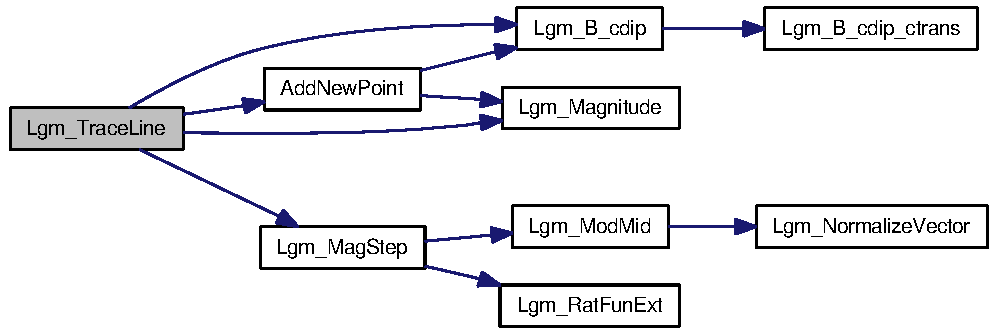
\includegraphics[width=257pt]{_trace_line_8c_3683689fb880f54289fd4600f8b7dfc9_cgraph}
\end{center}
\end{figure}


Here is the caller graph for this function:\nopagebreak
\begin{figure}[H]
\begin{center}
\leavevmode
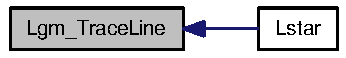
\includegraphics[width=101pt]{_trace_line_8c_3683689fb880f54289fd4600f8b7dfc9_icgraph}
\end{center}
\end{figure}
\hypertarget{_trace_line_8c_603527e81ecde7cb9495efc9bcb6d386}{
\index{TraceLine.c@{TraceLine.c}!Lgm\_\-TraceLine2@{Lgm\_\-TraceLine2}}
\index{Lgm\_\-TraceLine2@{Lgm\_\-TraceLine2}!TraceLine.c@{TraceLine.c}}
\subsubsection[{Lgm\_\-TraceLine2}]{\setlength{\rightskip}{0pt plus 5cm}int Lgm\_\-TraceLine2 ({\bf Lgm\_\-Vector} $\ast$ {\em u}, \/  {\bf Lgm\_\-Vector} $\ast$ {\em v}, \/  double {\em H0}, \/  double {\em MinDist}, \/  double {\em sgn}, \/  double {\em tol}, \/  int {\em AddBminPoint}, \/  {\bf Lgm\_\-MagModelInfo} $\ast$ {\em Info})}}
\label{_trace_line_8c_603527e81ecde7cb9495efc9bcb6d386}




Definition at line 340 of file TraceLine.c.

Here is the call graph for this function:\nopagebreak
\begin{figure}[H]
\begin{center}
\leavevmode
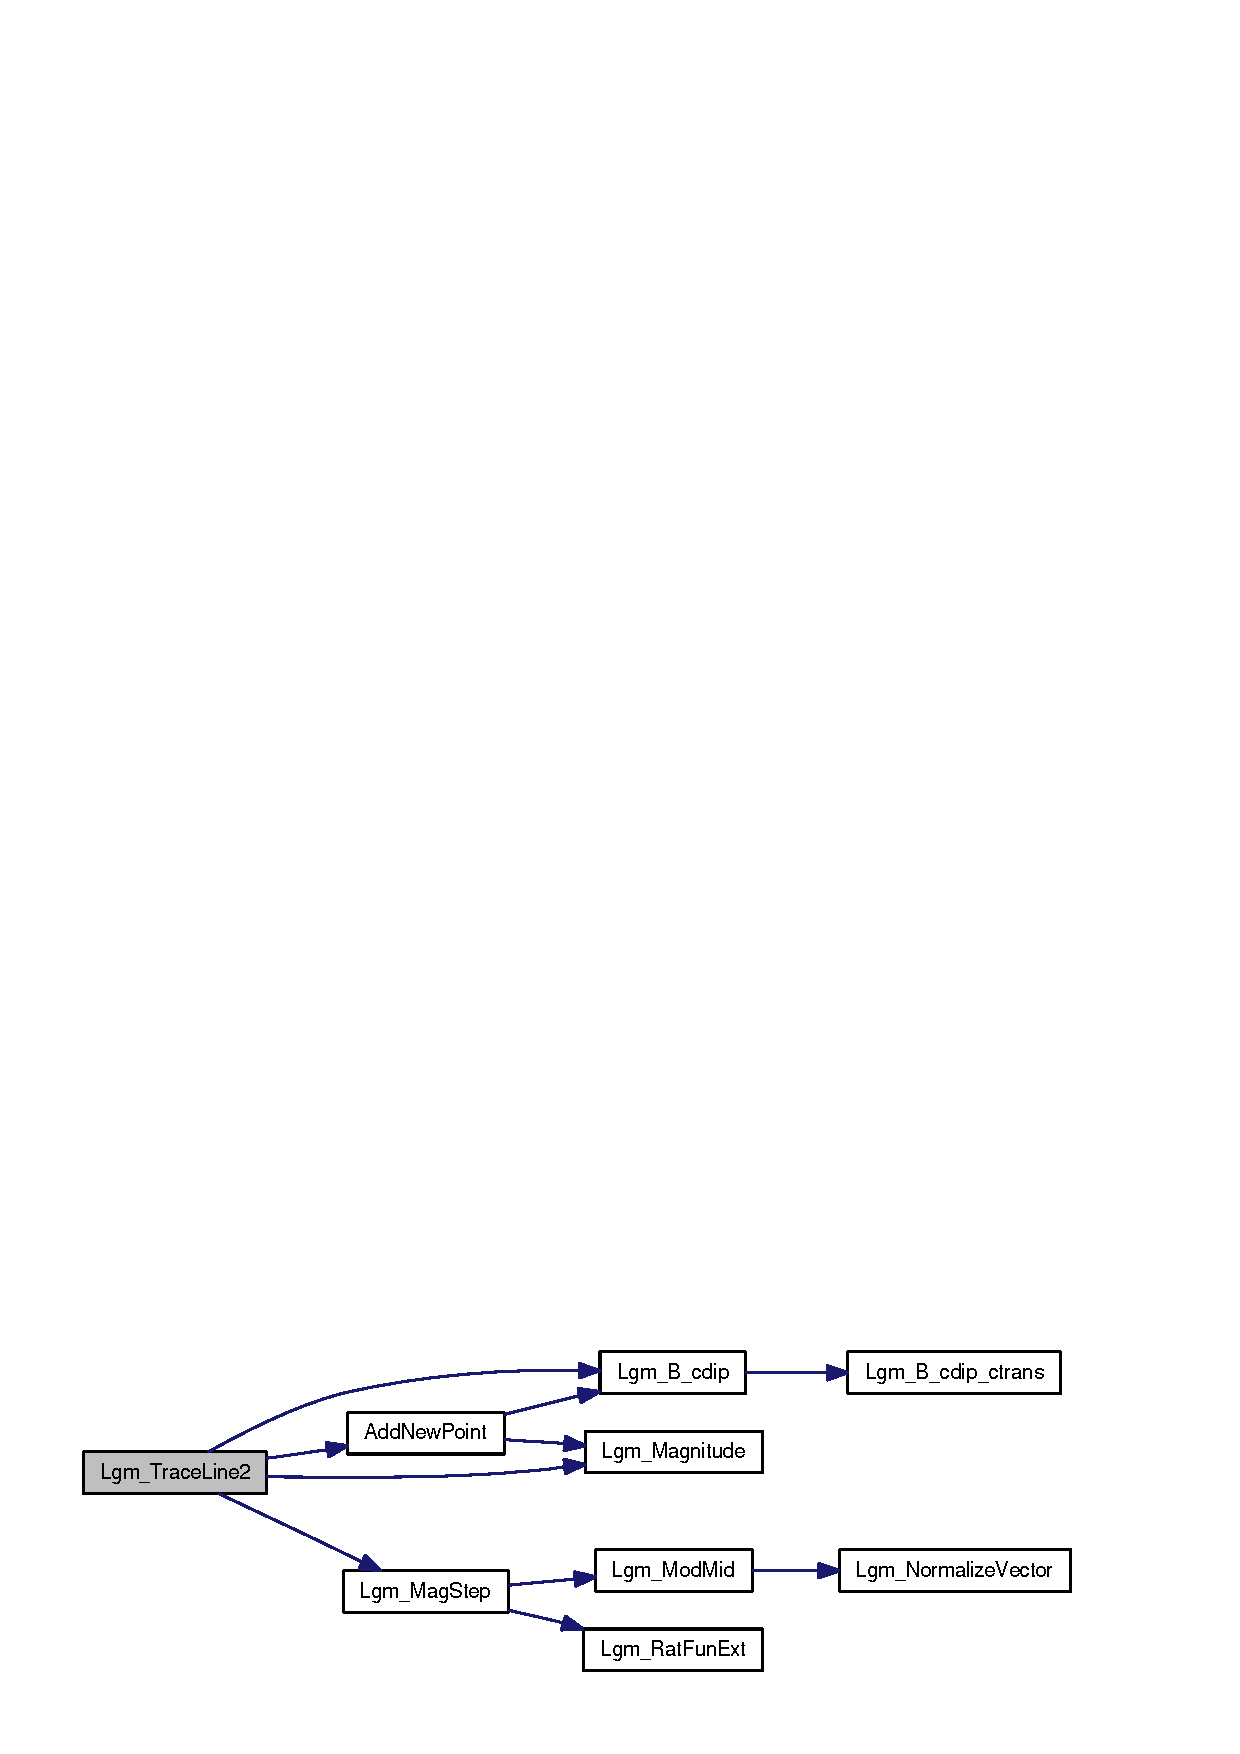
\includegraphics[width=259pt]{_trace_line_8c_603527e81ecde7cb9495efc9bcb6d386_cgraph}
\end{center}
\end{figure}


Here is the caller graph for this function:\nopagebreak
\begin{figure}[H]
\begin{center}
\leavevmode
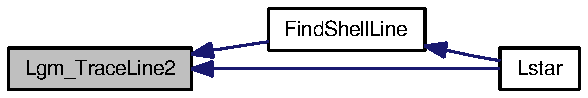
\includegraphics[width=159pt]{_trace_line_8c_603527e81ecde7cb9495efc9bcb6d386_icgraph}
\end{center}
\end{figure}
\hypertarget{_trace_line_8c_069290bbefbad1db8e625b9e8a0d3a5e}{
\index{TraceLine.c@{TraceLine.c}!ReplaceFirstPoint@{ReplaceFirstPoint}}
\index{ReplaceFirstPoint@{ReplaceFirstPoint}!TraceLine.c@{TraceLine.c}}
\subsubsection[{ReplaceFirstPoint}]{\setlength{\rightskip}{0pt plus 5cm}void ReplaceFirstPoint (double {\em s}, \/  double {\em B}, \/  {\bf Lgm\_\-Vector} $\ast$ {\em P}, \/  {\bf Lgm\_\-MagModelInfo} $\ast$ {\em Info})}}
\label{_trace_line_8c_069290bbefbad1db8e625b9e8a0d3a5e}




Definition at line 580 of file TraceLine.c.

Here is the call graph for this function:\nopagebreak
\begin{figure}[H]
\begin{center}
\leavevmode
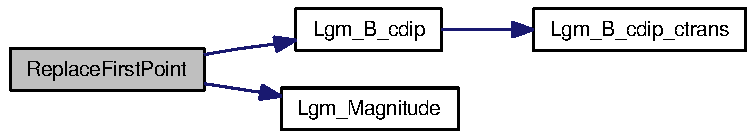
\includegraphics[width=199pt]{_trace_line_8c_069290bbefbad1db8e625b9e8a0d3a5e_cgraph}
\end{center}
\end{figure}


Here is the caller graph for this function:\nopagebreak
\begin{figure}[H]
\begin{center}
\leavevmode
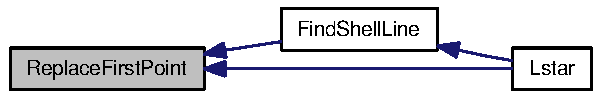
\includegraphics[width=162pt]{_trace_line_8c_069290bbefbad1db8e625b9e8a0d3a5e_icgraph}
\end{center}
\end{figure}
\hypertarget{_trace_line_8c_a82612dffc3edae2b3fce7cb94e435c0}{
\index{TraceLine.c@{TraceLine.c}!AddNewPoint@{AddNewPoint}}
\index{AddNewPoint@{AddNewPoint}!TraceLine.c@{TraceLine.c}}
\subsubsection[{AddNewPoint}]{\setlength{\rightskip}{0pt plus 5cm}void AddNewPoint (double {\em s}, \/  double {\em B}, \/  {\bf Lgm\_\-Vector} $\ast$ {\em P}, \/  {\bf Lgm\_\-MagModelInfo} $\ast$ {\em Info})}}
\label{_trace_line_8c_a82612dffc3edae2b3fce7cb94e435c0}




Definition at line 595 of file TraceLine.c.

Here is the call graph for this function:\nopagebreak
\begin{figure}[H]
\begin{center}
\leavevmode
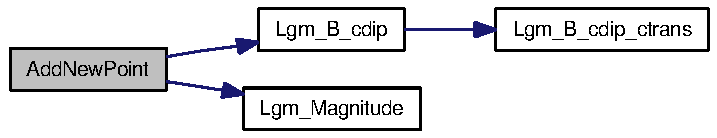
\includegraphics[width=190pt]{_trace_line_8c_a82612dffc3edae2b3fce7cb94e435c0_cgraph}
\end{center}
\end{figure}


Here is the caller graph for this function:\nopagebreak
\begin{figure}[H]
\begin{center}
\leavevmode
\includegraphics[width=219pt]{_trace_line_8c_a82612dffc3edae2b3fce7cb94e435c0_icgraph}
\end{center}
\end{figure}
\hypertarget{_trace_line_8c_a7175b98aed0d6f712ca66d532afe450}{
\index{TraceLine.c@{TraceLine.c}!InitSpline@{InitSpline}}
\index{InitSpline@{InitSpline}!TraceLine.c@{TraceLine.c}}
\subsubsection[{InitSpline}]{\setlength{\rightskip}{0pt plus 5cm}void InitSpline ({\bf Lgm\_\-MagModelInfo} $\ast$ {\em Info})}}
\label{_trace_line_8c_a7175b98aed0d6f712ca66d532afe450}




Definition at line 667 of file TraceLine.c.

Here is the caller graph for this function:\nopagebreak
\begin{figure}[H]
\begin{center}
\leavevmode
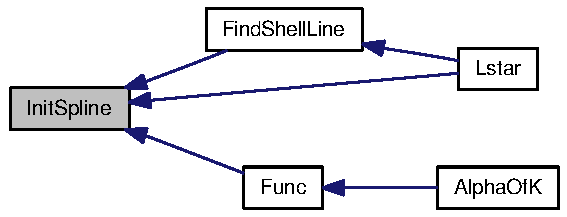
\includegraphics[width=154pt]{_trace_line_8c_a7175b98aed0d6f712ca66d532afe450_icgraph}
\end{center}
\end{figure}
\hypertarget{_trace_line_8c_e748e444fc7e684dcead584e1d002e8d}{
\index{TraceLine.c@{TraceLine.c}!FreeSpline@{FreeSpline}}
\index{FreeSpline@{FreeSpline}!TraceLine.c@{TraceLine.c}}
\subsubsection[{FreeSpline}]{\setlength{\rightskip}{0pt plus 5cm}void FreeSpline ({\bf Lgm\_\-MagModelInfo} $\ast$ {\em Info})}}
\label{_trace_line_8c_e748e444fc7e684dcead584e1d002e8d}




Definition at line 716 of file TraceLine.c.

Here is the caller graph for this function:\nopagebreak
\begin{figure}[H]
\begin{center}
\leavevmode
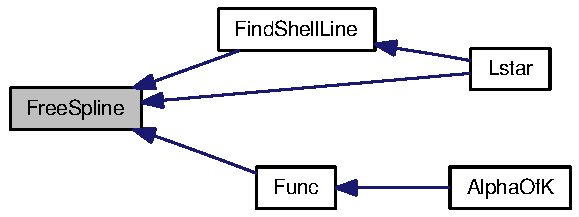
\includegraphics[width=157pt]{_trace_line_8c_e748e444fc7e684dcead584e1d002e8d_icgraph}
\end{center}
\end{figure}
\hypertarget{_trace_line_8c_be359d7bc7bae132a2e5bff78da3d9b2}{
\index{TraceLine.c@{TraceLine.c}!BofS@{BofS}}
\index{BofS@{BofS}!TraceLine.c@{TraceLine.c}}
\subsubsection[{BofS}]{\setlength{\rightskip}{0pt plus 5cm}double BofS (double {\em s}, \/  {\bf Lgm\_\-MagModelInfo} $\ast$ {\em Info})}}
\label{_trace_line_8c_be359d7bc7bae132a2e5bff78da3d9b2}




Definition at line 736 of file TraceLine.c.

Here is the call graph for this function:\nopagebreak
\begin{figure}[H]
\begin{center}
\leavevmode
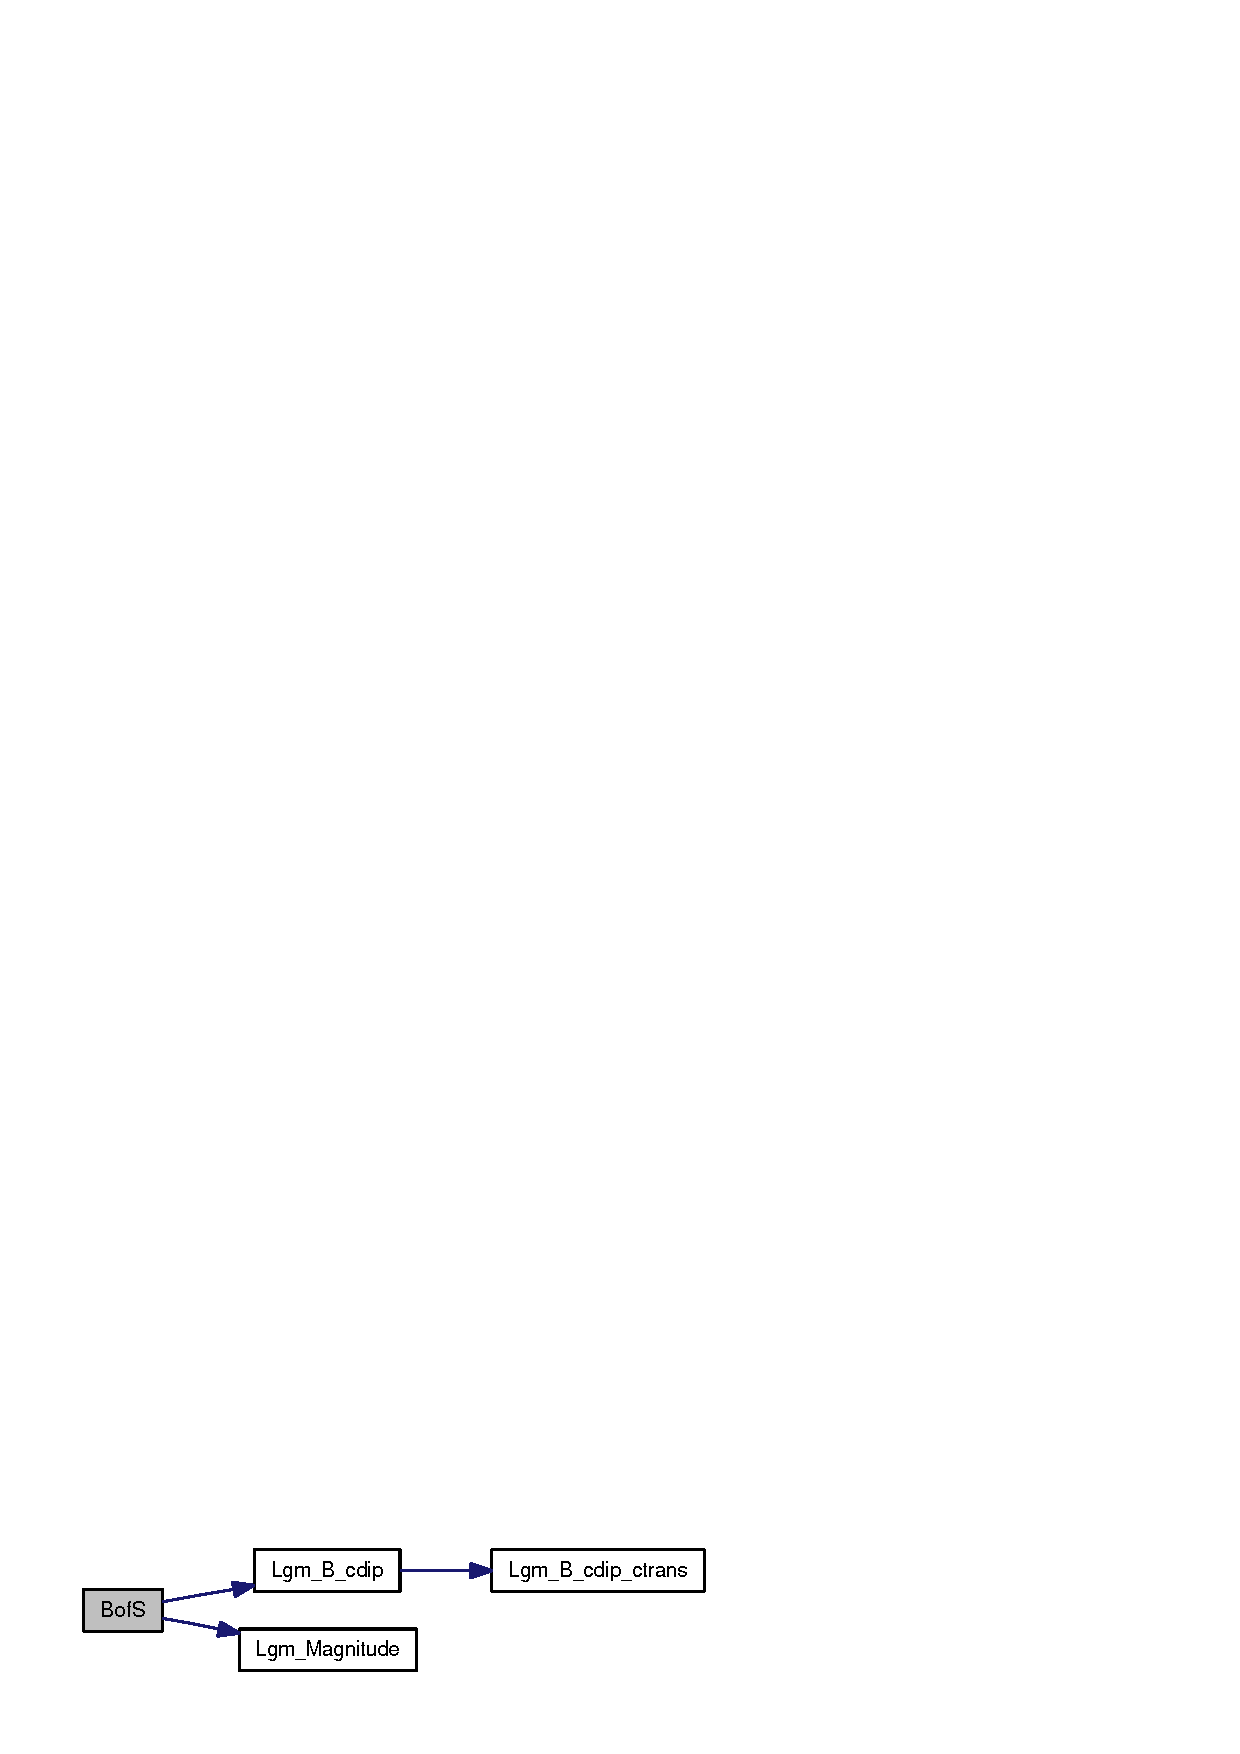
\includegraphics[width=171pt]{_trace_line_8c_be359d7bc7bae132a2e5bff78da3d9b2_cgraph}
\end{center}
\end{figure}


Here is the caller graph for this function:\nopagebreak
\begin{figure}[H]
\begin{center}
\leavevmode
\includegraphics[width=287pt]{_trace_line_8c_be359d7bc7bae132a2e5bff78da3d9b2_icgraph}
\end{center}
\end{figure}
\hypertarget{_trace_line_8c_d90887c3d7981a285406d4a15192ac44}{
\index{TraceLine.c@{TraceLine.c}!SofBm@{SofBm}}
\index{SofBm@{SofBm}!TraceLine.c@{TraceLine.c}}
\subsubsection[{SofBm}]{\setlength{\rightskip}{0pt plus 5cm}int SofBm (double {\em Bm}, \/  double $\ast$ {\em ss}, \/  double $\ast$ {\em sn}, \/  {\bf Lgm\_\-MagModelInfo} $\ast$ {\em Info})}}
\label{_trace_line_8c_d90887c3d7981a285406d4a15192ac44}




Definition at line 835 of file TraceLine.c.

Here is the call graph for this function:\nopagebreak
\begin{figure}[H]
\begin{center}
\leavevmode
\includegraphics[width=212pt]{_trace_line_8c_d90887c3d7981a285406d4a15192ac44_cgraph}
\end{center}
\end{figure}
